\documentclass[./main.tex]{subfiles}

\begin{document}

本章我们将解决几个有趣的问题,同时尝试用函数式的方式来解决这些问题。

\subsection*{运算逆波兰表示法}

学校里学习的数学表达式都是中置(infix)表示法,比如 $10 - (4 + 3) * 2$,其中 $+$,$*$,$-$就是中置算子。在 Haskell
中就像是\acode{+}或者\acode{elem}那样。这种写法对于人类来说便于阅读和理解,但是缺点就是必须用括号来描述运算的优先级。

逆波兰法(Reverse Polish notation form)是另一种数学的表示法,上述表达式用 RPN 表达就是 $10\ 4\ 3\ +\ 2\ *\ -$。
可以想象成堆叠,从左往右阅读算式,每当碰到一个数值就把它堆上堆叠。当碰到一个算子,就把两个数值从堆叠上拿下来,运算完成后
再将结果堆上堆叠。

\begin{figure}[h]
  \centering
  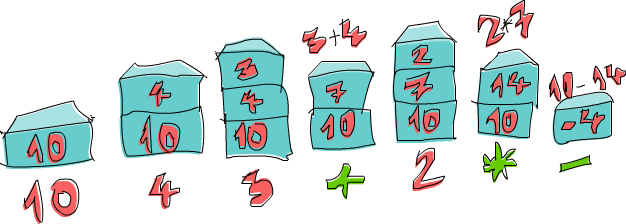
\includegraphics[width=0.9\textwidth]{\subfix{./images/rpn.png}}
\end{figure}

\begin{anote}
  在实现一个函数之前,更重要的是思考其类型声明。在 Haskell 中,一个函数的类型声明能告诉我们很多函数的信息,感谢强壮的
  类型系统。
\end{anote}

现在来写一个 Haskell 函数用于处理 RPN 运算式:

\begin{lstlisting}[language=Haskell]
  import Data.List

  solveRPN :: (Num a) => String -> a
  solveRPN expression = head (foldl foldingFunction [] (words expression))
      where   foldingFunction stack item = ...
\end{lstlisting}

首先是接受一个表达式,通过\acode{words}将其转换为各个列表中的项。再用\acode{foldl}函数接受的\acode{foldingFunction}
处理堆叠,且\acode{[]}作为累加器,初始状态即为空的堆叠,最后用\acode{head}获取最终堆叠的单个值。通过 point-free 风格
取出括号,再用\acode{where}声明函数\acode{foldingFunction}。

\begin{lstlisting}[language=Haskell]
  solveRPN :: (Num a, Read a) => String -> a
  solveRPN = head . foldl foldingFunction [] . words
    where
      foldingFunction (x : y : ys) "*" = (x * y) : ys
      foldingFunction (x : y : ys) "+" = (x + y) : ys
      foldingFunction (x : y : ys) "-" = (y - x) : ys
      foldingFunction xs numberString = read numberString : xs
\end{lstlisting}

\acode{foldingFunction}展开成四个模式匹配,从第一个开始尝试匹配,三种算符情况下取头部两个元素直接进行计算,非三种算符时
则进入最后一个匹配,将输入视为可转换的数值字符串(如果\acode{read}失败则抛出异常)进行堆叠。测试:

\begin{lstlisting}[language=Bash]
  ghci> solveRPN "10 4 3 + 2 * -"
  -4
  ghci> solveRPN "2 3 +"
  5
  ghci> solveRPN "90 34 12 33 55 66 + * - +"
  -3947
  ghci> solveRPN "90 34 12 33 55 66 + * - + -"
  4037
  ghci> solveRPN "90 34 12 33 55 66 + * - + -"
  4037
  ghci> solveRPN "90 3 -"
  87
\end{lstlisting}

现在修改一下函数使其可以接受更多的算符,为了简化使其返回类型为\acode{Float}:

\begin{lstlisting}[language=Haskell]
  solveRPN :: String -> Float
  solveRPN = head . foldl foldingFunction [] . words
    where
      foldingFunction (x : y : ys) "*" = (x * y) : ys
      foldingFunction (x : y : ys) "+" = (x + y) : ys
      foldingFunction (x : y : ys) "-" = (y - x) : ys
      foldingFunction (x : y : ys) "/" = (y / x) : ys
      foldingFunction (x : y : ys) "^" = (y ** x) : ys
      foldingFunction (x : xs) "ln" = log x : xs
      foldingFunction xs "sum" = [sum xs]
      foldingFunction xs numberString = read numberString : xs
\end{lstlisting}

\begin{lstlisting}[language=Haskell]
  ghci> solveRPN "2.7 ln"
  0.9932518
  ghci> solveRPN "10 10 10 10 sum 4 /"
  10.0
  ghci> solveRPN "10 10 10 10 10 sum 4 /"
  12.5
  ghci> solveRPN "10 2 ^"
  100.0
  ghci> solveRPN "43.2425 0.5 ^"
  6.575903
\end{lstlisting}

最后就是注意该函数并没有错误容忍的能力,假设输入的表达式并不合理,那么程序便会崩溃。因此将函数类型改为
\acode{solveRPN :: String -> Maybe Float}则更为合理,我们会在学习 monads 的时候再来进行实现。当然我们现在也可以
实现,只不过会有一大堆检查\acode{Nothing}的动作(可以使用\acode{reads}来看看一次 read 是否成功)。

\subsection*{路径规划}

\begin{figure}[h]
  \centering
  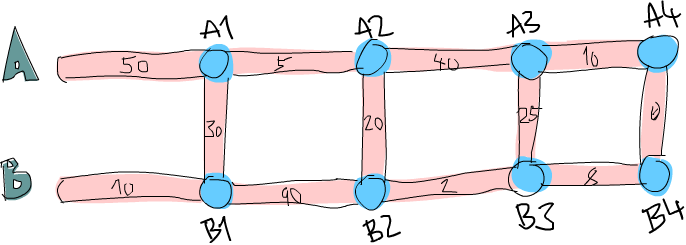
\includegraphics[width=0.9\textwidth]{\subfix{./images/roads_simple.png}}
\end{figure}

使用 Haskell 数据类型来描述问题。一种做法是起始点与交叉点作为图的节点,想象起点也有一条长度为 1 的虚拟道路连接,
每个交叉点都连接对面节点,同时也连到下一个交叉点,除了最后一个节点。数据类型如下:

\begin{lstlisting}[language=Haskell]
  data Node = Node Road Road | EndNode Road
  data Road = Road Int Node
\end{lstlisting}

一个节点要么是普通节点,其包含了去往另一个主路的信息以及去往下一个节点(相同主路)的信息;要么是一个终点,其仅包含了去往
另一个主路的信息。一个路则是包含了长度信息,以及其指向的节点。

另一种做法就是用\acode{Maybe}来代表往下一个节点(相同主路)的信息。每个节点都有指到另一条主路节点的路径,但只有不是终点的
节点才有指向下一个节点(相同主路)的路。

\begin{lstlisting}[language=Haskell]
  data Node = Node Road (Maybe Road)
  data Road = Road Int Node
\end{lstlisting}

实际上,每次检查只会检查三条路径的长度:道路 A 的部分,道路 B 的部分,以及它们相连的部分。当观察 A1 与 B1 的最短路径时,
只需考虑第一组的三个部分,即花费 50,10 以及 30。因此道路系统可以由四组数据来表示:$50, 10, 30$,$5, 90, 20$,
$40, 2, 25$ 以及 $10, 8, 0$。

让我们的数据类型越简单越好,不过这样已经是极限了:

\begin{lstlisting}[language=Haskell]
  data Section = Section {getA :: Int, getB :: Int, getC :: Int} deriving (Show)
  type RoadSystem = [Section]
\end{lstlisting}

那么 Heathrow 去 London 的道路系统便可这样表示:

\begin{lstlisting}[language=Haskell]
  heathrowToLondon :: RoadSystem
  heathrowToLondon = [Section 50 10 30, Section 5 90 20, Section 40 2 25, Section 10 8 0]
\end{lstlisting}

剩下需要做的就是实现方案。首先引入\acode{Label}类型,作为一个枚举包含了\acode{A},\acode{B}或\acode{C},另外就是一个
类型同义词\acode{Path}:

\begin{lstlisting}[language=Haskell]
  data Label = A | B | C deriving (Show)
  type Path = [(Label, Int)]
\end{lstlisting}

我们的函数\acode{optimalPath}其类型声明就应该是\acode{optimalPath :: RoadSystem -> Path}。那么在调用
\acode{heathrowToLondon}之后,其应该返回如下路径:

\begin{lstlisting}[language=Haskell]
  [(B,10),(C,30),(A,5),(C,20),(B,2),(B,8)]
\end{lstlisting}

在手动解答时,有一个步骤我们在不断的重复,那就是检查 A 与 B 的最佳路径以及当前的 section,产生新的 A 与 B 的最佳路径。
例如,最开始的最佳路径是\acode{[]}与\acode{[]},看到\acode{Section 50 10 30}后得到新的到 A1 最佳路径为
\acode{[(B,10),(C,30)]},而到 B1 的最佳路径是\acode{[(B,10)]}。如果吧这个步骤看做一个函数,那么便是接受一对
路径以及一个 Section,并产生出新的一对路径。因此函数类型为\acode{(Path, Path) -> Section -> (Path, Path)}。

\begin{anote}
  类型为\acode{(Path, Path) -> Section -> (Path, Path)}非常的有用,因为可以被二元函数 left fold 所使用,其需要的
  类型就是\acode{a -> b -> a}。
\end{anote}

\begin{lstlisting}[language=Haskell]
  roadStep :: (Path, Path) -> Section -> (Path, Path)
  roadStep (pathA, pathB) (Section a b c) =
    let priceA = sum $ map snd pathA
        priceB = sum $ map snd pathB
        forwardPriceToA = priceA + a
        crossPriceToA = priceB + b + c
        forwardPriceToB = priceB + b
        crossPriceToB = priceA + a + c
        newPathToA =
          if forwardPriceToA <= crossPriceToA
            then (A, a) : pathA
            else (C, c) : (B, b) : pathB
        newPathToB =
          if forwardPriceToB <= crossPriceToB
            then (B, b) : pathB
            else (C, c) : (A, a) : pathA
     in (newPathToA, newPathToB)
\end{lstlisting}

这里发生了什么?首先是基于先前 A 的最佳解计算道路 A 的最佳解,B 同理。使用\acode{sum \$ map snd pathA},如果
\acode{pathA}是\acode{[(A,100),(C,20)]},那么\acode{priceA}变为\acode{120}。如果直接从之前的 A 去往下一个
A 节点,那么\acode{forwardPriceToA}则是要付的成本;\acode{crossPriceToA}则是先前在 B 上前往 A 所付出的成本。

记住,路径是相反的,因此要从右向左读。

\begin{anote}
  \textbf{优化小技巧}:当\acode{priceA = sum \$ map snd pathA}时,我们在计算每个步骤的成本。如果我们实现的
  \acode{roadStep}类型是\acode{(Path, Path, Int, Int) -> Section -> (Path, Path, Int, Int)},那么就
  不必这么做。这里的整数类型代表 A 与 B 上的最小成本。
\end{anote}

现在有了接受一对路径以及一个 section 并返回最佳路径的函数,我们可以用 left fold 来使用它。将\acode{([],[])}
以及第一个 section 代入至\acode{roadStep}中就可以得到一对最佳路径,然后再将这个最佳路径以及新的 section 代入至
\acode{roadStep}就可以得到下一个最佳路径。以此类推,我们可以用以实现\acode{optimalPath}:

\begin{lstlisting}[language=Haskell]
  optimalPath :: RoadSystem -> Path
  optimalPath roadSystem =
    let (bestAPath, bestBPath) = foldl roadStep ([], []) roadSystem
     in if sum (map snd bestAPath) <= sum (map snd bestBPath)
          then reverse bestAPath
          else reverse bestBPath
\end{lstlisting}

测试:

\begin{lstlisting}[language=Haskell]
  ghci> optimalPath heathrowToLondon
  [(B,10),(C,30),(A,5),(C,20),(B,2),(B,8),(C,0)]
\end{lstlisting}

符合预期!现在要做的是从标准输入读取文本形式的道路系统,并将其转换成\acode{RoadSystem},然后再用\acode{optimalPath}
来运行一遍即可。

首先是一个接受列表并将其切成同样大小的 group 的函数,例如当参数是\acode{[1..10]}时,\acode{groupsOf 3}则应该返回
\acode{[[1,2,3],[4,5,6],[7,8,9],[10]]}:

\begin{lstlisting}[language=Haskell]
  groupsOf :: Int -> [a] -> [[a]]
  groupsOf 0 _ = undefined
  groupsOf _ [] = []
  groupsOf n xs = take n xs : groupsOf n (drop n xs)
\end{lstlisting}

接下来是 main 函数:

\begin{lstlisting}[language=Haskell]
  main = do
  contents <- getContents
  let threes = groupsOf 3 (map read $ lines contents)
      roadSystem = map (\[a, b, c] -> Section a b c) threes
      path = optimalPath roadSystem
      pathString = concatMap (show . fst) path
      pathPrice = sum $ map snd path
  putStrLn $ "The best path to take is: " ++ pathString
  putStrLn $ "The price is: " ++ show pathPrice
\end{lstlisting}

创建一个\acode{paths.txt}文件:

\begin{lstlisting}
  50
  10
  30
  5
  90
  20
  40
  2
  25
  10
  8
  0
\end{lstlisting}

执行:

\begin{lstlisting}[language=Haskell]
  $ cat paths.txt | runhaskell heathrow.hs
  The best path to take is: BCACBBC
  The price is: 75
\end{lstlisting}

\end{document}
